\section{Implementation}
\label{sec:implementations}

In this section we give our implementation of functional arrays (sequences). We show the correctness of our implementation. We show that \get{} and \set{} on leaf sequences require constant work, and \get{} and \set{} on interior sequences require bounded work. As such, our implementation matches the structural dynamics of a versioned data structure, and we can use the evaluational dynamics we derived to analyze costs of parallel programs involving sequences.

We give SML-like code for our implementation. In our implementation we construct and manipulate mutable arrays (henceforth called arrays). We assume that an array of size $n$ can be created with $n$ work on a single processor machine and $\log{n}$ work on a machine with an unbounded number of processors. new$(n, v)$ creates a new array of size $n$ with $v$ at each index. tabulate$(n, f)$ creates a new array of size $n$ which for all $i$ contains $f(i)$ at the $i^{\text{th}}$ index. sub$(A,i)$ evaluates to the $i^{\text{th}}$ element of array $A$ with constant work. update$(A, i, v)$ mutates index $i$ of array $A$ to have value $v$ with constant work.

Our implementation assumes an atomic compare and swap function \func{cmpswap}. \func{cmpswap}$(a$ : int ref, $v$ : int, $v'$ : int$)$ : bool is a single atomic operation. It compares the value at $a$ to $v$, and if and only if they are the same sets the value at $a$ to $v'$ and returns true, otherwise it returns false.

We assume a $p$-processor parallel machine model. For our proofs of correctness, we assume a sequentially consistent memory model. When analyzing costs, we assume that all processors are synchronized with respect to a global clock. At each time step, as many processors as possible execute a single pending instruction.

\subsection{Pusharray Implementation}

We use an auxiliary data structure, pusharrays, to store log entries. Conceptually, pusharrays are lists that support 3 functions. Suppose we have a pusharray $A$. $\tpush{}(A,e)$ inserts entry $e$, $\tsize{}(A)$ returns the number of entries inserted, $\tget(A,i)$ returns the $i^{\text{th}}$ entry inserted. Note that \get{} is only defined between indices 0 and $\tsize{}(A)-1$. All operations have amortized constant work.

Pusharrays can be used semi-concurrently. At most one thread can execute instructions in \push{} at any time, but multiple threads can call \size{} and \get{}. The type definition for pusharrays is given below.

\begin{lstlisting}[language=ML]
type capacity = int
type size = int
type 'a pusharray = (capacity ** size 
                              ** 'a array) ref
\end{lstlisting}

The pusharray's array stores the entries inserted into the pusharray. Size represents the number of entries inserted and capacity represents the size of the array. If the pusharray does not have the capacity for more insertions, it copies all entries to an array that is twice as large. The implementation for \push{} is given below.

\begin{lstlisting}[language=ML]
val push : 'a pusharray ** 'a -> unit
fun push$(A \mbox{ as } \mbox{ref}(c,s,D), v)$ =
  if $c = s$ then 
    let val $c' = 2 \times c$
       val $D'$ = Array.new$(c', v)$
    in copyArray$(D,D')$;
       update$(D',s,v)$;
       A := $(c',s+1,D')$
    end
  else 
    update$(D, s, v)$;
    A := $(c, s+1, D)$
\end{lstlisting}

\size{} simply returns the size attribute of the pusharray, and \get{}$(A,i)$ returns the $i^{\text{th}}$ index in the pusharray's data array. Intuitively, the reason that pusharrays are needed for our sequence implementation is that they are linearizable ~\cite{linearizability} given that different calls to \push{} (on the same pusharray) do not overlap.

\subsection{Sequence Implementation}
Our sequence implementation keeps a value array of the most recent values, which represents the values at a leaf node of the version tree. For each index of the array we store a change-log that keeps track of values at interior nodes of the version tree. The type definition for sequences is given below.

\begin{lstlisting}[language=ML]
type version = int
type 'a logs = ('a pusharray) array
type 'a arraydata = version ref ** 'a array 
                                ** 'a logs
type 'a sequence = version ** 'a arraydata
\end{lstlisting}

Note that multiple sequences can reference the same arraydata. Figure \ref{fig:new_array_A} visualizes a newly created sequence $A$.

\begin{figure}[!ht]
\centering
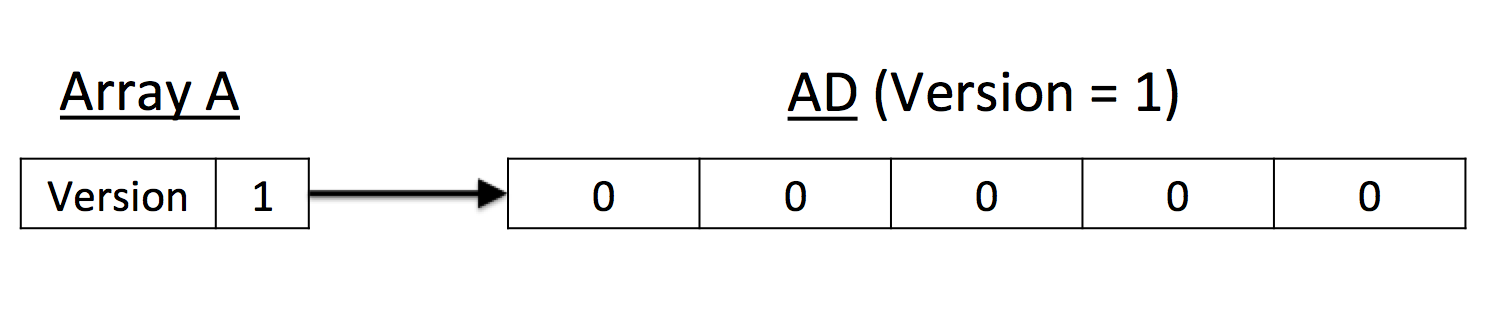
\includegraphics[scale=0.3]{new_array_A}
\nocaptionrule \caption{A = \new{}(5, 0)}
\label{fig:new_array_A}
\end{figure}

The implementation of \new{} is given below.

\begin{lstlisting}[language=ML]
val new : int ** 'a -> 'a sequence
fun new(size, init) =
  (1, (ref 1, Array.new(size, init), 
    tabulate(size, 
      fn _ => Pusharray.new$(0, \mbox{init})$)))
\end{lstlisting}

\set{} uses a compare and swap to increment the arraydata's version so that only one thread can modify an arraydata at any point in time. If the compare and swap is successful (which means the sequence is a leaf sequence), a log entry is inserted and the value array is mutated. Otherwise, the values in the sequence are copied over to produce a new arraydata. The new arraydata will have empty logs at each index. Note that the values are not directly copied into the new arraydata from the value array, we need to call \get{} at each index of the sequence when getting the values. 

The ordering of the instructions in \set{} is critical. If the vals array is modified before the log entry is inserted then a \get{} evaluated between the 2 instructions could evaluate to the wrong value.

Figure \ref{fig:set_old_array} visualizes \set{}s on interior and leaf sequences.
\begin{figure}[!ht]
\centering
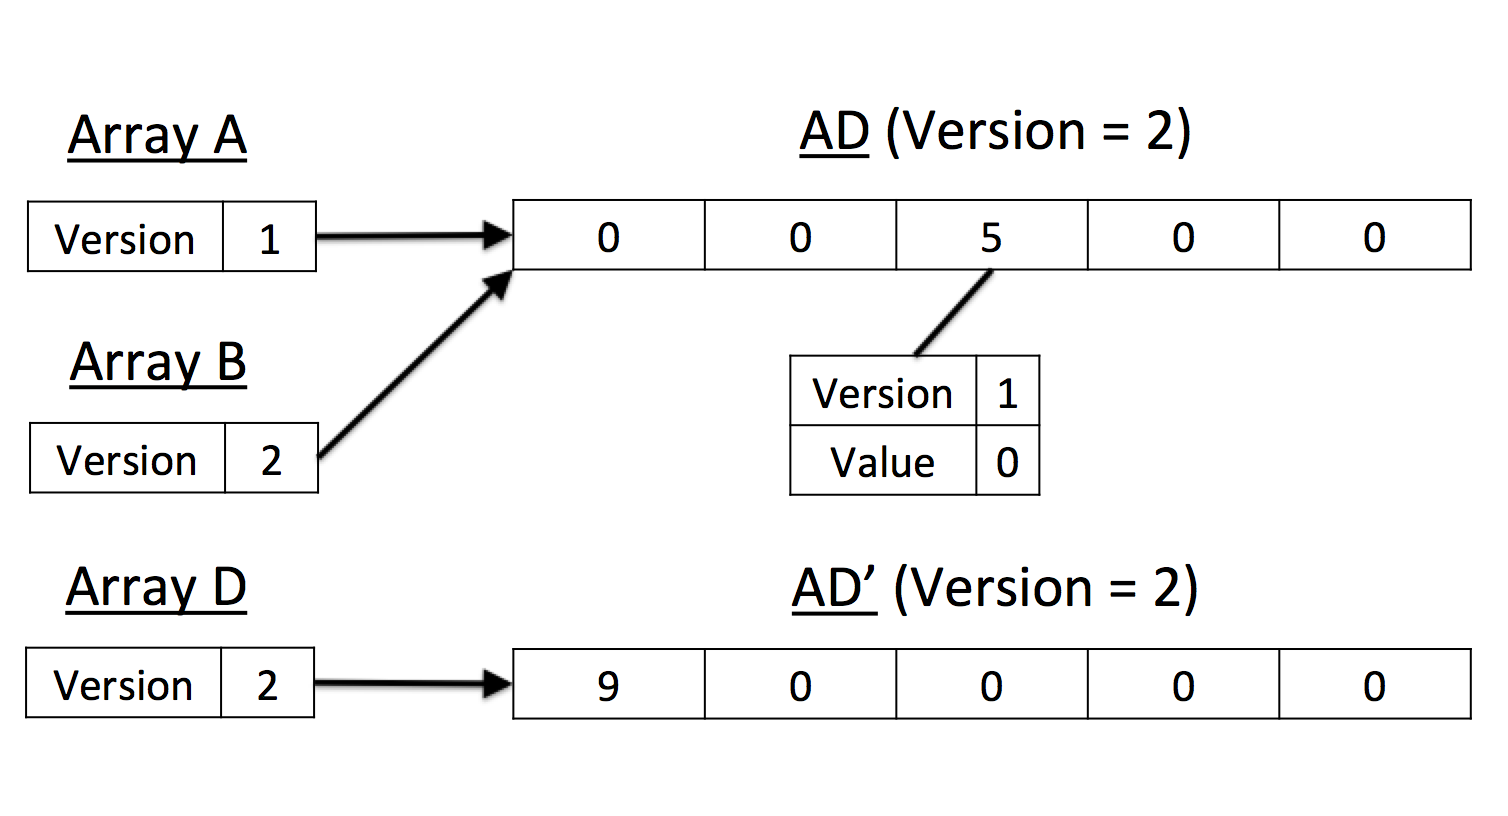
\includegraphics[scale=0.3]{set_old_array}
\nocaptionrule \caption{$B = \tset(A, 2, 5)$ changes the value array and adds a log entry. Then $D = \tset(A, 0, 9)$ creates $AD'$ because $A$ is interior.}
\label{fig:set_old_array}
\end{figure}

The implementation of \set{} is given below.

\begin{lstlisting}[language=ML,escapechar=|]
val set : 'a sequence ** int ** 'a -> 'a sequence
fun set$((V,(V_r, A, L)),i,v)$ = 
  if not(cmpswap$(V_r, V, (V+1))$)|\label{line:set-cmpswap}| orelse
     (!$V_r \bmod \mbox{length}(A) = 0$) then
    let val $A'$ = getFarrayValues$((V,(V_r, A, L)))$
       val $L'$ = emptyLogs(size($A$))
    in update$(A', i, v)$; $(1, (\mbox{ref }1, A', L')$ 
    end
  else
    Pusharray.push$(\mbox{sub}(L,i),(V,\mbox{sub}(A,i)))$; |\label{line:start-cmpswap}|
    update$(A, i, v)$;
    $(V+1, (V_r, A, L))$ |\label{line:end-cmpswap}|
\end{lstlisting}

\get{}$(A,i)$ first loads the value $v$ at the $i^{\text{th}}$ index of the value array. If the sequences' version and corresponding arraydata's version match (meaning that the sequence is a leaf sequence), then \get{} evaluates to $v$. If the log at index $i$ is empty or all versions in the log at index $i$ are less than the sequence version, then \get{} evaluates to $v$. Otherwise, \get{} binary searches the log at index $i$ for the value corresponding to the least version $\geq$ the sequence's version.

As in \set{}, the ordering of the instructions in \get{} is important. In particular, index $i$ of the value array must be loaded before the versions are compared or the logs are examined. If the versions are compared first and a \set{} is evaluated between the 2 instructions, the \set{} might modify the value array and cause the \get{} to evaluate to the wrong value.

The implementation of \get{} is given below.

\begin{lstlisting}[language=ML,escapechar=|]
val get : 'a sequence ** i -> 'a
fun get$((V, (V_r, A, L)),i)$ =
let val guess = sub$(A,i)$ |\label{line:load-value}|
   val $l$ = sub$(L, i)$
   val $n$ = Pusharray.size$(l)$
in if $V = \;!V_r$ then guess |\label{line:get-version-check}|
   else if $n = 0$ then guess |\label{line:log-empty}|
   else
      let val $(V', \_)$ = Pusharray.get$(l, n-1)$
      in if $V' < V$ then guess |\label{line:log-small}|
        else valueAtLeastVersionGeq$(l,V)$ |\label{line:binary-search}|
      end
\end{lstlisting}

\subsection{Target Language}

For our proofs we give a more formal definition of the target language in which we implement sequences\footnote{Our target language is different from the SML-like code used in the code samples. This for clarity of our code samples. It is easy to translate our code samples to our target language.}. The target language extends the source language to support mutable references and compare and swap. The structural dynamics of the target language is given by the following judgement, where $(\pi, \mu)$ is the memory and $(\pi', \mu')$ is the memory after the step has been taken,
$$(\pi, \mu), e \to_T (\pi', \mu'), e'$$

For simplicity we assume all sequences and arraydatas are int sequences and int arraydatas. To avoid dealing with overflow issues, we assume that all integers in the target language are unbounded. Sequences are represented as $\&l$ where the label $l$ indexes into the store $\pi$.

The memory contains an immutable store $\pi$ that maps labels to $(\lambda, *k)$ where $\lambda$ is an integer version number and $k$ is an index into $\mu$. Intuitively, $\pi$ contains all the sequences created so far in the evaluation of the expression. New key-value pairs can be inserted into $\pi$ but existing mappings cannot be modified. The memory also contains a mutable store $\mu$ that maps labels to values $(V, A, L)$ of type int arraydata. 

For concision we do not give the full dynamics of our target language. As examples, we give the rules for creating a new arraydata, pushing a log entry, and compare and swap. Let $a_n$ denote an array of $n$ $a$s and let $\{\}$ denote an empty $(\mbox{int} * \mbox{int})$ pusharray.
$$\frac{n \text{ int val} \;\;\; k \not\in L(\mu)}{(\pi, \mu), \mbox{\func{newad}}(n) \to_T (\pi, \mu[k \mapsto (0, 0_n, \{\}_n)]), *k}\text{ (new-ad)}$$

$$\frac{V, V' \text{ int val} \;\;\; \mu[k] = (V, A, L)}{(\pi, \mu), \mbox{\func{cmpswap}}(*k, V, V') \to_T (\pi, \mu[k \mapsto (V', A, L)]), \text{true}}\text{ (cas-true)}$$

$$\frac{V, V' \text{ int val} \;\;\; \mu[k] \neq (V, A, L)}{(\pi,\mu), \text{\func{cmpswap}}(*k, V, V') \to_T (\pi,\mu), \text{false}}\text{ (cas-false)}$$

$$\frac{\begin{gathered}\mu[k] = (V, A, L) \;\;\; i, V', v \text{ int val} \;\;\; \\ L[i] = (p_1, ..., p_n) \;\;\; L' = L[i \mapsto (p_1, ..., p_n, (V',v))]\end{gathered}}{(\pi,\mu), \text{\func{push}}(*k, i, (V', v)) \to (\pi,\mu[k \mapsto (V, A, L')]), *k} \text{ (push)}$$

In the source language, evaluating \new{}, \get{}, and \set{} involves a single step. In the target language, \new{}, \get{}, and \set{} are function calls to our implementation. Evaluating the function calls requires multiple steps. Let $C(\tnew{})$, $C(\tget{})$, $C(\tset{})$ be the implementation (that is, the lambda expression) for \new{}, \get{}, and \set{} respectively. 

The following rules show the evaluation of \get{} and \set{} in the target. \get{} is simply substituted with its implementation. For \set{}, we use a \set{}' ``wrapper" so that the sequence \set{} evaluates to can be added to the store $\pi$ in the end-set rule. We keep track of the sequences created so we can show invariants on sequences in our proof of correctness.

$$\frac{i \text{ int val}}{(\pi, \mu), \tget{}(\&l, i) \to_T (\pi, \mu), C(\tget{})(\&l, i)} \text{ (get)}$$

$$\frac{i, v \text{ int val}}{(\pi,\mu), \text{\set{}}(\&l, i, v) \to_T (\pi, \mu), \text{\set{}}'(C(\text{\set{}})(\&l, i, v))} \text{ (start-set)}$$

$$\frac{(\pi, \mu), e \to_T (\pi',\mu'), e'}{(\pi,\mu), \text{\set{}}'(e) \to_T (\pi',\mu'), \text{\set{}}'(e')} \text{ (eval-set)}$$

$$\frac{l \not\in L(\pi)}{(\pi, \mu), \text{\set{}}'((V,*k)) \to_T (\pi[l \mapsto (V, *k)], \mu), \&l} \text{ (end-set)}$$

The rules for \new{} are similar to \set{}. As in the source structural dynamics, either side of a fork-join expression in the target can take a step. This makes the target structural dynamics non-deterministic. However, because \get{} and \set{} involve multiple steps, the target has a greater number of possible interleavings than the source.

\begin{definition}
A transition sequence in the target language is a sequence of memory stores $[(\pi_0, \mu_0), ..., (\pi_n, \mu_n)]$ and expressions $[e_0, ..., e_n]$ such that for all $0 \leq i < n$, $(\pi_i, \mu_i), e_i \to_T (\pi_{i+1}, \mu_{i+1}), e_{i+1}$. We say that $(\pi_0, \mu_0), e_0 \to^*_T (\pi_n, \mu_n), e_n$ or $(\pi_0, \mu_0), e_0, \to^n_T (\pi_n, \mu_n), e_n$.
\end{definition}

An expression $e$ in the source language is compiled to an expression $e'$ in the target and then executed according to the target's dynamics. Since the source language is a subset of the target language, $e = e'$. In other words an expression $e$ in the source language can be viewed as an expression in the target.

We show that our implementation of sequences in the target correctly implements the source. The non-atomicity of \set{} and \get{} means that we cannot appeal to standard parametricity theorems for our proofs.

\subsection{Proof of Correctness}

The full correctness proof follows along the lines of~\cite{concurrent-logical} and~\cite{concurrent-logical2}. We concentrate here on the critical parts, involving \new{}, \get{}, and \set{}. We give a rely-guarantee style argument~\cite{rely-guarantee} for the correctness of our implementation (for integer sequences).

We show invariants on the memory store and constraints on the possible ways that the memory store can evolve in a valid target program. Given these invariants and constraints, we show that \new{}, \get{}, and \set{} behave the same way in the source and target. The tricky part of the proof is setting up the invariants and theorems---the proofs follow from extensive but straightforward casework.

\begin{definition}
(Valid memories) Consider memory store $(\pi, \mu)$. Consider arbitrary label $l \in L(\pi)$ and suppose $\pi[l] = (\lambda, k)$. We say $(\pi, \mu)$ is valid at $l$ if the following hold.
\begin{enumerate}
\item $k \in L(\mu)$. Assuming this is true, let $\mu[k] = (V, A, L)$.
\item $0 \leq \lambda \leq V$
\item For all $i$ and $0 \leq j < \text{\func{len}}(L[i])$ if $L[i][j] = (V', v)$ then $V' < V$
\item For all $i$ and $0 \leq j < k < \text{\func{len}}(L[i])$, if $L[i][j] = (V_1, v_1)$ and $L[i][k] = (V_2, v_2)$ then $V_1 < V_2$
\end{enumerate}
We say $(\pi, \mu)$ \emph{valid} if for all $l \in L(\pi)$, $(\pi, \mu)$ is valid at $l$. 
\end{definition}

\begin{theorem}
Let $e$ be an expression in the source language. Suppose that $(\{\}, \{\}), e \to^*_T (\pi, \mu), e'$. Then $(\pi, \mu)$ \emph{valid}.
\end{theorem}

\begin{proof}
(Outline) By induction on the length of the transition sequence taking $(\{\}, \{\}), e$ to $(\pi, \mu), e'$. For the base case, verify that each condition holds for $(\{\}, \{\})$. 

Our IH is that that the theorem holds for all transition sequences of length $n$. We then consider an arbitrary transtion sequence of length $n+1$. From the IH, the first $n$ steps leads to a valid memory state. We then case on all possible modifications that the $n+1^{\text{th}}$ step can make to memory. Showing properties (1) to (3) is straightforward. To prove property (4), we need to appeal to a lemma that different executions of lines~\ref{line:start-cmpswap} to~\ref{line:end-cmpswap} in the implementation of \set{} on the same arraydata cannot overlap. The lemma holds because of property (2) and the compare and swap.
\end{proof}

\begin{definition}
(Memory transformations) Consider $(\pi, \mu), (\pi', \mu')$ \emph{valid} \footnote{Note that the relation is only defined for valid memory states.}. Consider arbitrary label $l$ with $l \in L(\pi)$ and $l \in L(\pi')$. Suppose that $\pi[l] = (\lambda, k)$ and $\pi'[l] = (\lambda', k')$. We say that $(\pi, \mu) \leq (\pi, \mu)$ at $l$ if the following hold.
\begin{enumerate}
\item $\lambda = \lambda'$ and $k = k'$ (in other words, values in $\pi$ are immutable). Assuming this is true, let $\mu[k] = (V, A, L)$ and $\mu'[k] = (V', A', L')$.
\item $V \leq V'$. In other words, the versions are non-decreasing.
\item For all $i$, \func{len}$(L[i]) \leq$ \func{len}$(L'[i])$ and for all $i, j$ with $0 \leq j < $ \func{len}$(L[i])$, $L[i][j] = L'[i][j]$. Intuitively, this means that logs can only be extended, existing entries cannot be overwritten.
\item If \func{len}$(L[i]) <$ \func{len}$(L'[i])$ then $L'[$\func{len}$(L[i])] = (V'', A[i])$ where $V \leq V''$.
\item For all $i$, if $A[i] \neq A'[i]$ then $\lambda < V'$ and exists $0 \leq j < \text{\func{len}}(L'[i])$ with $L'[i][j] = (V'', A[i])$ and $\lambda \leq V''$.
\end{enumerate}
We say that $(\pi, \mu) \leq (\pi', \mu')$ if $L(\pi) \subseteq L(\pi')$ and for all $l$ s.t. $l \in L(\pi)$ and $l \in L(\pi')$, $(\pi, \mu) \leq (\pi', \mu')$ at $l$.
\end{definition}

\begin{lemma}
(Reflexivity) If $(\pi, \mu)$ \emph{valid} then $(\pi, \mu) \leq (\pi, \mu)$. 
\end{lemma}

\begin{lemma}
(Transitivity) If $(\pi_0, \mu_0) \leq (\pi_1, \mu_1)$ and $(\pi_1, \mu_1) \leq (\pi_2, \mu_2)$ then $(\pi_0, \mu_0) \leq (\pi_2, \mu_2)$.
\end{lemma}

\begin{theorem}
Let $e$ be an expression in the source language. Suppose that $(\{\}, \{\}), e \to^*_T (\pi, \mu), e'$ and $(\pi, \mu), e' \to^*_T (\pi', \mu'), e''$. Then $(\pi, \mu) \leq (\pi', \mu')$.
\end{theorem}

\begin{proof}
(Outline) By induction on the length of the transition sequence taking $(\pi, \mu), e'$ to $(\pi', \mu'), e''$. The base case is trivial. For the inductive step case on the possible modifications the implementation can make to memory and then use transitivity of $\leq$.
\end{proof}

\begin{definition}
Suppose $A_S, A_T$ val. We say that $\sigma, A_S \sim (\pi, \mu), A_T$ if $A_S, A_T$ have the same length and for all valid $i$, $\sigma, \tget{}(A_S, i) \to^* \sigma', v$ and $(\pi, \mu), \tget{}(A_T, i) \to^*_T (\pi', \mu'), v$ for some $v$ int val.
\end{definition}

\begin{lemma}
\label{preservation-lemma}
(Monotonicity) If $\sigma, A_S \sim (\pi, \mu), A_T$ and $(\pi, \mu) \leq (\pi', \mu')$ then $\sigma, A_S \sim (\pi', \mu'), A_T$.
\end{lemma}

Because the target language supports concurrency, the memory store might be modified (by other evaluations of \new{} and \set{}) while \new{}, \get{}, and \set{} are being evaluated. To account for this we define concurrent transition sequences.

\begin{definition}
A \emph{concurrent transition sequence} $\tau$ in the target is a left sequence of memories $[(\pi_0,\mu_0), ..., (\pi_{n-1},\mu_{n-1})]$, right sequence of memories $[(\pi_0',\mu_0'), ..., (\pi_{n-1}',\mu_{n-1}')]$ and expressions $[e_0, ..., e_n]$ with $(\pi_i,\mu_i), e_i \to_T (\pi_i',\mu_i'), e_{i+1}$ for all $i$, and $(\pi_i', \mu_i') \leq (\pi_{i+1}, \mu_{i+1})$ for all $0 \leq i < n-1$. We say that $\tau$ takes $(\pi_0, \mu_0), e_0$ to $(\pi_{n-1}',\mu_{n-1}'), e_{n-1}'$.
\end{definition}

\begin{theorem}
(\new{}) Suppose that for some $A_S, A_T$ \emph{val}, \\$\sigma, \tnew{}(n, v) \to^* \sigma', A_S$ and $(\pi, \mu), \tnew{}(n,v) \to^*_T (\pi', \mu'), A_T$. Then $\sigma', A_S \sim (\pi', \mu'), A_T$.
\end{theorem}

\begin{proof}
Because the logs are empty, \get{} on every index of $A_T$ evaluates to 0. Similarly, \get{} on every index of $A_S$ evaluates to 0.
\end{proof}

\begin{theorem}
\label{thm-get}
(\get{}) Suppose that $\sigma, A_S \sim (\pi, \mu), A_T$. Fix $i$ \emph{int val}. Suppose that $\sigma, \tget{}(A_S, i) \to^* \sigma’, v$ where $v$ \emph{int val}. Let $e_0 = \tget{}(A_T, i)$ and suppose that $(\pi, \mu) \leq (\pi_0, \mu_0)$. Consider a concurrent transition sequence from $(\pi_0, \mu_0), e_0$ to $(\pi_{n-1}', \mu_{n-1}'), e_n$ with $e_n$ \emph{int val}. Then $e_n = v$.
\end{theorem}

\begin{proof}
(Outline) We case on the line that the implementation of \get{} returns. There are 4 cases: lines \ref{line:get-version-check}, \ref{line:log-empty}, \ref{line:log-small}, and \ref{line:binary-search}. In each case, we show that $e_n$ is the same as the value $(\pi, \mu), \tget{}(A_T, i)$ evaluates to. Since $\sigma, A_S \sim (\pi, \mu), A_T$, this is the same value that $\sigma, \tget{}(A_S, i)$ evaluates to, which implies $e_n = v$.

The first case is on line \ref{line:get-version-check} in the implementation of \get{}, where \emph{guess} is returned if the version of the sequence and arraydata are the same. Since sequence versions are immutable, arraydata versions are non-decreasing, and sequence versions are $\leq$ array data versions, the sequence and arraydata versions are also the same on line \ref{line:load-value}. From the implementation of \get{}, if the entire \get{} was evaluated atomically on line \ref{line:load-value}, it would evaluate to \emph{guess}. By lemma~\ref{preservation-lemma} this means that \emph{guess} and $v$ are the same.

The other cases on lines \ref{line:log-empty} and \ref{line:log-small} are similar. In the last case, \get{} involves a binary search on the logs. The theorem follows for the binary-search case from property (3) in memory transformations (logs can only be extended) and property (4) in valid memories (versions in a log are strictly increasing).
\end{proof}

\begin{theorem}
(\set{}) Suppose that $\sigma, A_S \sim (\pi,\mu), A_T$. Fix $i, v$ \emph{int val}. Suppose that $\sigma, \tset{}(A_S, i) \to^* \sigma', A_S'$ where $A_S'$ \emph{val}. Let $e_0 = \tset{}(A_T, i, v)$ and suppose that $(\pi, \mu) \leq (\pi_0, \mu_0)$. Consider a concurrent transition sequence from $(\pi_0, \mu_0), e_0$ to $(\pi_{n-1}', \mu_{n-1}'), e_n$ with $e_n$ \emph{val}. Then $\sigma', A_S' \sim (\pi_{n-1}', \mu_{n-1}'), e_n$.
\end{theorem}

\begin{proof}
(Outline) Case on whether the compare and swap in \set{} evaluates to true or false.

If it evaluates to false, then the implementation calls \get{} at each index of $A_T$ and creates a new arraydata in $\mu$. In this case $\sigma', A_S' \sim (\pi_{n-1}', \mu_{n-1}'), e_n$ follows from theorem~\ref{thm-get}.

If it evaluates to true, then from lemma~\ref{preservation-lemma} $A_S$ and $A_T$ are related when the compare and swap evaluates. In the source, \set{}$(A_S, i, v)$ evaluates to $A_S[i \mapsto v]$. In the target, suppose that $A_T = \&l$, $\pi[l] = (\lambda, k)$ and $\mu[k] = (V, A, L)$. As argued before, different executions of lines~\ref{line:start-cmpswap} to~\ref{line:end-cmpswap} in the implementation of \set{} on the same arraydata cannot overlap. So in the target, the implementation sets $\mu[k] = (V+1,A[i \mapsto v], L')$ for some $L'$ and returns $\&l'$ s.t. $\pi[l'] = (V+1, k)$. Going through the definition of $\sim$ this gives us $\sigma', A_S' \sim (\pi_{n-1}', \mu_{n-1}'), \&l'$.

\end{proof}

\begin{theorem}
(Bounded cost) There exists $k$ s.t. if $A_T$ has size $n$ then there does not exist $(\pi, \mu)$ \emph{valid} and a concurrent transition sequence of length $> kn$ starting at either $(\pi, \mu), \tget{}(A_T, i)$ or $(\pi, \mu), \tset{}(A_T, i, v)$ for all $i, v$ \emph{int val}.
\end{theorem}

\begin{proof}
(Outline) Because we copy the contents of a sequence after $n$ updates, where $n$ is the size of the sequence, for some $k$ independent of $n$, \set{} involves at most $kn$ steps, and \get{} involves at most $k\log{n}$ steps.
\end{proof}

\subsection{Interleaved Cost Bounds}

We want to show that work done in the interleaved structural dynamics is an upper bound for the work done in the implementation. We first sketch a linearizability-type result~\cite{linearizability}.

Consider the execution $E$ of a program. We assume a sequentially consistent model of computation. Consider a sequential execution $S$ of instructions in $E$ that produces the same result as $E$. 

Consider any \get{} in the sequential execution $S$. From the previous subsection, the result that the program evaluates to does not depend on how the instructions in the \get{} are interleaved. Consider line \ref{line:get-version-check} in \get{} where the version of the array is compared with its arraydata. If the versions match then \get{} involves a constant amount of work. Otherwise, in the worst case \get{} involves a binary search on $n$ elements, where $n$ is the size of the array. This takes work proportional to $\log{n}$ \footnote{\set{} also copies the sequence data once every $n$ times the version number is increased, but the copying is amortized constant time.}.

So the execution $S$ is upper bounded (in cost) by an execution where the entire \get{} is evaluated atomically at the instruction where the versions of the array and arraydata are compared, where the \get{} has constant work if the version check succeeds and $\log{n}$ work if the check fails.

Similarly, consider any \set{} in the sequential execution $S$. From the previous subsection, the result that the program evaluates to does not depend on how the instructions in the \set{} are interleaved. Consider line \ref{line:set-cmpswap} in \set{} which involves a compare and swap on the arraydata's version. If the compare and swap is successful then \set{} involves a constant amount of work. Otherwise, in the worst case \set{} involves copying over $n$ elements, where $n$ is the size of the array. This takes work proportional to $n$.

So the execution $S$ is upper bounded (in cost) by an execution where the entire \set{} is evaluated atomically at the compare and swap instruction, where the \set{} has constant work if the compare and swap succeeds and $n$ work if the compare and swap fails.

We can trivially assume that \new{} is evaluated atomically since none of the effects of \new{} are observable until it finishes evaluating, and \new{} always takes time proportional to the size of the array being created.

We then define a relation between sequences in the source and target. $\sigma, A_S$ in the source and $(\pi, \mu), A_T$ in the target are related if \get{} evaluates to the same value at all indices, and $A_S$ is a leaf sequence if and only if $\lambda = V$ where $A_T = \&l$, $\pi[l] = (\lambda, k)$, and $\mu[k] = (V, A, L)$. We show that the relation is preserved by \new{} and \set{} and that costs of operations in the source are an upper bound for operations in the target for related sequences. Since the execution was transformed so that \new{}, \get{}, and \set{} evaluate atomically, we can then prove and apply a parametricity theorem to show that programs in the source and target evaluate to the same value.

\subsection{Parallel Cost Bounds}

Next, we sketch the case where we have an unbounded number of processors. In the worst case, \get{} involves a binary search on $n$ elements, where $n$ is the size of the array. This takes $\log{n}$ time on a machine with an unbounded number of processors. In the worst case, \set{} involves copying $n$ array elements and $n$ log entries where $n$ is the size of the array. In a machine with an unbounded number of processors, the copying can be done in $\log{n}$ time. Similarly, \new{} can execute in $\log{n}$ time on a machine with an unbounded number of processors. Note that the implementation of \new{}, \get{}, and \set{} are wait-free so these costs are independent of what other threads are doing.

It follows that we can use the evaluational dynamics to compute the work $W$ and span $S$ of evaluating an expression $e$ in our source language. We can then use theorem~\ref{thm:brent} to get that the cost of evaluating $e$ on a $p$-processor machine is $\leq c(\frac{W}{P} + S\log{P})$ for some constant $c$ independent of $e$.

